% standard LaTeX packages
\documentclass[11pt,a4paper]{article}

\usepackage[utf8]{inputenc}
\usepackage[T1]{fontenc}
\usepackage[english]{babel}
\usepackage[margin=3cm]{geometry}
\usepackage{parskip}
\usepackage{xifthen}
\usepackage{placeins} %Floatbarrier
\usepackage{graphicx} %package to manage images
\usepackage{subcaption}

% math packages
\usepackage{mathtools,amsfonts,amssymb,mathdots}
\usepackage{siunitx}

\usepackage[rightcaption]{sidecap}

\newcommand{\dd}[1]{\mathrm{d}#1} %numbering
% plotting and tables
\usepackage{tikz}
\usepackage{pgfplots}
\usepackage{pgfplotstable}
\usepackage{caption}
% other packages
\usepackage{filecontents}


\begin{document}

\title{Prosjekt 3: Modell av solsystemet ved hjelp av ordinære differensialligninger }
\author{Live Wang Jensen \\ Joseph Knutson}
\date{\today}

\maketitle

\begin{abstract}
I dette prosjektet har vi gradvis simulert et solsystem i objektorientert kode. Hovedfokus er på hvordan velocity Verlet  metoden
bevarer energi og angulærmoment, samtidig som dens globale feil er mye mindre enn Eulers metode. Selv om Verlet metoden koster mer CPU-tid enn Euler så vil Verlet alltid holde seg innenfor en viss radius, isteden for å drifte ut i verdensrommet.
Vi bestemte jordens eksperimentelle unnslipningshastighet til å ligge mellom 8.75 og 8.90 AU/yr, mens den teoretiske verdien var 8.89 AU/yr. I tillegg har vi demonstrert hvordan generell relativitet påvirker Merkurs perihelpresesjon.
\end{abstract}

\tableofcontents

\clearpage
\section{Introduksjon}
Målet med dette prosjektet er å utvikle en kode som kan simulere solsystemet ved hjelp av den populære \textit{velocity Verlet} algoritmen. Vi kommer til å se at dette systemet kan beskrives ved hjelp av to koblede differensialligninger, og at disse kan løses numerisk på flere ulike måter. Koden vi har brukt for å simulere dette systemet er objekt-orientert, noe som gjør det enkelt å innføre nye planeter og bytte mellom ulike løsningsmetoder. Vi skal ta for oss Eulers metode og velocity Verlet metoden, og sammenligne disse på flere områder. Spesielt skal vi se på antall FLOPS og CPU-tiden til de to metodene. Vi skal også se på hvor godt de to metodene konserver ulike fysiske størrelser som angulærmoment og mekanisk energi. \\

I første del av prosjektet skal vi se på et forenklet solsystem med jorden som eneste planet kretsende rundt solen. Dette gjøres for å teste selve algoritmen og se om alt fungerer. Her skal vi teste både Eulers metode og velocity Verlet metoden, men videre skal vi kun bruke Verlet metoden, da denne er mye mer stabil. Dette vil våre observasjoner av feil og energi/angulærmomentbevaring bevise. Etterhvert skal vi bestemme jordens unnslipninghastighet både eksperimentelt og eksakt, og sammenligne disse resultatene med hverandre. Videre innføres Jupiter, slik at vi får et trelegemeproblem. Vi skal da flytte origo fra solen til systemets massesenter. I tillegg skal vi gi solen en initiell hastighet som er slik at systemets totale bevegelsesmengde er null. Til slutt innfører vi en modell av et fullstendig solsystem med alle planeter, og ser på hvordan dette oppfører seg som funksjon av tiden. \\

I tillegg skal vi se på Merkurs bane og hvordan den påvirkes av den relativistiske tyngdekraften. Dersom vi trekker fra alle klassiske påvirkniger fra den observerte verdien til Merkurs perihelpresesjon, ender vi opp med en perihelpresesjon på 43'' (arc seconds) per århundre. I vår simulering skal vi se nærmere på dette, og se om vi kan komme frem til det samme resultatet.

\section{Teori}
Det er kun tyngdekraften som virker på systemet vårt. Newtons tyngdelov sier at tyngdekraften som virker mellom to legemer, er proporsjonal med produktet av deres masse, og omvendt proporsjonal med kvadratet av avstanden mellom dem [5]. Dersom vi skal se på tyngdekraften som virker mellom solen og jorden, kan loven kan uttykkes på følgende måte:
\begin{equation}
F_G = \frac{GM_{\odot}M_{Earth}}{r^2}
\end{equation}
hvor $M_{\odot}$ er solens masse, $M_{Earth}$ er jordens masse, $G$ er gravitasjonskonstanten og $r$ er avstanden mellom jorden og solen. Vi antar at massen til solen er mye større enn massen til jorden, slik at vi kan se bort fra tyngdekraften som virker på solen i jord-sol-systemet. \\

Dersom vi antar at jordens bane rundt solen ligger i $xy$-planet, kan vi bruke Newtons andre lov til å finne
\begin{equation}
 \frac{d^2x}{dt^2}=\frac{F_{G,x}}{M_{\mathrm{Earth}}}
\end{equation}
og 
\begin{equation}
\frac{d^2y}{dt^2}=\frac{F_{G,y}}{M_{\mathrm{Earth}}}
\end{equation}

hvor $F_{G,x}$ og $F_{G,y}$ er $x$ og $y$ komponentene til tyngdekraften. I dette prosjektet skal vi bruke astronomiske enheter (AU). Èn astronomisk enhet er altså den gjennomsnittlige avstanden mellom jorden og solen, 1 AU = 1.5$\times10^{11}$m. I tillegg bruker vi enheten år i stedet for sekunder til å måle tiden med. I vårt system er solens masse skalert slik at $M_{\odot} = 1$. Massen til alle de andre planetene skaleres derfor i forhold til solmassen, for eksempel vil $M_{Earth,skalert} = M_{\odot}/M_{Earth}$. 


\section{Løsningsmetoder}
Vi kan beregne jordens bane rundt solen ved å bruke enten Eulers metode eller velocity Verlet algoritmen til å løse de ordinære differensialligningene gitt ovenfor. Dersom vi antar at jorden beveger seg i en sirkulær bane rundt solen, vet vi i følge Newtons andre lov at tyngkraften som virker på jorden må være
\[F_G = \frac{M_{Earth}v^2}{r} = \frac{GM_{\odot}M_{Earth}}{r^2}  \]
siden $a = v^2/r$ for en sirkulær bane, hvor $v$ er jordens hastighet. Denne ligningen kan brukes til å vise at 
\[v^2r = GM_{\odot} = 4\pi^2 AU^3/yr^2  \]

\subsection{Euler}
Vi kan diskretisere ligningene gitt ovenfor slik at vi kan sette opp en algoritme for å løse ligningene ved hjelp av Eulers metode. Dersom vi har en funksjon $y$, kan vi finne ut hvordan funksjonen ser ut i et tidssteg $y_{i+1}$ ved hjelp av det tidligere tidssteget $y_i$:
\[y_{i+1} = y(t= t_i + h) = y(t_i) + h\Delta(t_i, y_i(t_i)) + O(h^{p+1}) \]
hvor $h = (b - a)/N$ er steglengden, $N$ er antall tidssteg, $a$ og $b$ er integrasjonsgrensen og $O(h^{p+1})$ er feilen i beregningen vår. $\Delta$ representerer alle de deriverte av funksjonen vår $y$:
\[\Delta(t_i, y_i(t_i)) = (y'(t_i) + ... + y^{(p)}(t_i)\frac{h^{p-1}}{p!} )  \]
Hvis vi definerer
\[y'(t_i) = f(t_i, y_i) \]
og minker $\Delta$ til å kun inneholde den førstederiverte av $y$, får vi
\[y_{i+1} = y(t_i) + hf(t_i,y_i) + O(h^2)  \]
og 
\[t_{i+1} = t_i + h \]
som sammen utgjør Eulers metode. Legg merke til at vi for hvert tidssteg får en feil på $O(h^2)$. Dette gir oss en global feil på $N\cdot O(h^2) \approx O(h)$  [7]. Eulers metode er altså ikke å anbefale hvis vi ønsker nøyaktighet i beregningene, men kan være nyttig dersom vi ønsker et førsteintrykk av hvordan løsningen kan se ut. \\

Et eksempel på hvordan dette kan implementeres i C++ vises i figur \ref{euler}. Her er \texttt{Euler} en funksjon i klassen med samme navn. Funksjonen starter med å hente funksjonen \texttt{calculateForcesAndEnergy()} fra klassen vår \texttt{SolarSystem}, som inneholder alle de nødvendige metodene for å simulere solsystemet, bortsett fra integrasjonsmetodene. Inne i for-løkken beregnes legemenes posisjon og hastighet ved hjelp av Eulers algoritme.

\FloatBarrier
\begin{figure}[!ht]
\begin{center}
  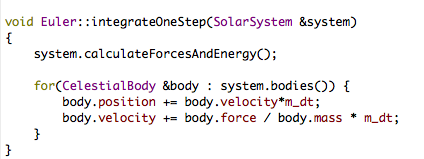
\includegraphics[width = 100mm]{euler.png}\\
  \caption{Eksempel på hvordan Eulers algoritme kan implementeres i en klasse i C++. Koden er hentet fra filen \texttt{euler.cpp}.}   \label{euler}
  \end{center}
  \end{figure}
\FloatBarrier


\subsection{Velocity Verlet}
En annen metode å løse differensialligningene på er Verlet metoden. Denne populære algoritmen er både numerisk stabil og enkel å implementere. Dersom vi tar for oss Newtons andre lov som en andre ordens differensialligning, som i én dimensjon kommer på formen
\[ m \frac{d^2x}{dt^2} = F(x,t) \]
Denne kan skrives om til to \textit{koblede} differensialligninger
\[\frac{dx}{dt} = v(x,t) \quad og \quad \frac{dv}{dt} = F(x,t)/m = a(x,t) \]
I Tayorutviklingen
\begin{equation}
x(t+h) = x(t) + hx^{(1)}(t) + \frac{h^2}{2}x^{(2)}(t) + O(h^3)
\label{1}
\end{equation}
kjenner vi den andrederiverte via Newtons andre lov, $x^{(2)} = a(x,t)$. Dersom vi legger til Taylorutviklingen for $x(t-h)$ i ligning \ref{1}, ender vi opp med 
\[x_{i+1} = 2x_i - x_{i-1} + h^2x_i^{(2)} + O(h^4) \]
hvor $x_{i\pm 1} = x(t_i \pm h)$ og $x_i = x(t_i)$. Feilen her går som $O(h^4)$, siden alle de odde leddene kansellerer i addisjonen [7]. Hastigheten er ikke direkte inkludert i ligningen, siden $x^{(2)}$ er kjent. Dersom vi trenger hastigheten, kan vi finne den ved å bruke ligningen
\[x_i^{(1)} = \frac{x_{i+1} - x_{i+1}}{2h} + O(h^2) \]
Hastigheten har altså en feil på $O(h^2)$. Legg merke til at algoritmen for posisjonen $x$ for $i=0$ trenger den ikke-eksisterende verdien $x_{-1}$ for å starte. Dette problemet unngås i \textbf{velocity Verlet} metoden. Taylorutviklingen til posisjonen er gitt som
\[x_{i+1} = x_i + hx_i^{(1)} + \frac{h^2}{2}x_i^{(2)} + O(h^3) \]
mens Taylorutviklingen til hastigheten er 
\[v_{i+1} = v_i + hv_i^{(1)} + \frac{h^2}{2}v_i^{2} + O(h^3) \]
Ved hjelp av Newtons andre lov har vi et analytisk uttrykk for den deriverte til hastigheten, nemlig
\[ v_i^{(1)} = \frac{d^2x}{dt^2}|_i = \frac{F(x_i, t_i)}{m} \]

Dersom vi adderer dette til Taylorutviklingen til akselerasjonen
\[v_{i+1}^{(1)} = v_i^{(1)} + hv_i^{(2)} + O(h^2) \]
og ser bort fra de høyere ordens leddene etter den andrederiverte av hastigheten, får vi 
\[hv_i^{(2)} \approx v_{i+1}^{(1)} - v_i^{(1)}  \]
Vi kan nå skrive om Taylorutviklingen til hastigheten som
\[ v_{i+1} = v_i + \frac{h}{2}\left( v_{i+1}^{(1)} + v_i^{(1)} \right) + O(h^3)  \]

Det vi ender opp med til slutt er den berømte \textbf{velocity Verlet} algoritmen:
\[x_{i+1} = x_i + hv_i + \frac{h^2}{2}v_i^{(1)} + O(h^3)  \]
\[v_{i+1} = v_i + \frac{h}{2} \left( v_{i+1}^{(1)} + v_i^{(1)} \right) + O(h^3)  \]

Implementasjonen finnes i filen \texttt{velocityverlet.cpp}, og et lite utsnitt av denne algortimen vises i figur \ref{vv}. Funksjonen \texttt{VelocityVerlet} starter med å initialisere kreftene som virker på systemet ved hjelp av funksjonen \texttt{calculateForcesAndEnergy}, før den bruker velocity Verlet metoden til å beregne legmenes hastighet og posisjon. Etter at dette er gjort, oppdateres kreftene før hastigheten beregnes igjen.

\FloatBarrier
\begin{figure}[!ht]
\begin{center}
  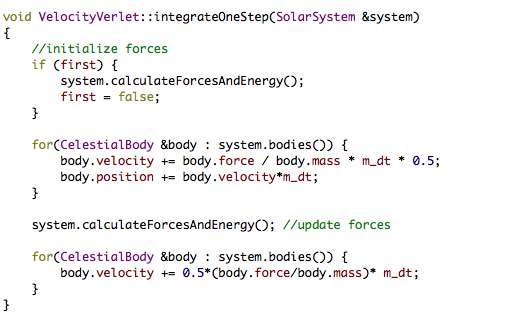
\includegraphics[width = 100mm]{vv.png}\\
  \caption{Eksempel på hvordan velocity Verlet algoritmen kan implementeres i en klasse i C++. Koden er hentet fra filen \texttt{velocityverlet.cpp}.}   \label{vv}
  \end{center}
  \end{figure}
\FloatBarrier

\section{Resultater}
\subsection{Konservering}
Energien er konservert ved bruk av Velocity Verlet, men ved bruk av Euler skjer det skumple ting.
Pga. Eulers akkumulerende feil ser det ut som at et arbeid blir påført systemet. Etter en hundreårs simulering av jorda er hverken angulærmoment eller mekanisk energi bevart.
Velocity Verlet derimot, står med glans. Enten systemet er tolegemet (Jorda og Sola), eller trelegemet (Jorda, Jupiter og Sola), så er energien og angulærmomentet bevart. Se figur \ref{ang1} og \ref{ang2}.\\

\FloatBarrier
\begin{figure}[!ht]
\centering
\begin{subfigure}{.50\textwidth}
  \centering
  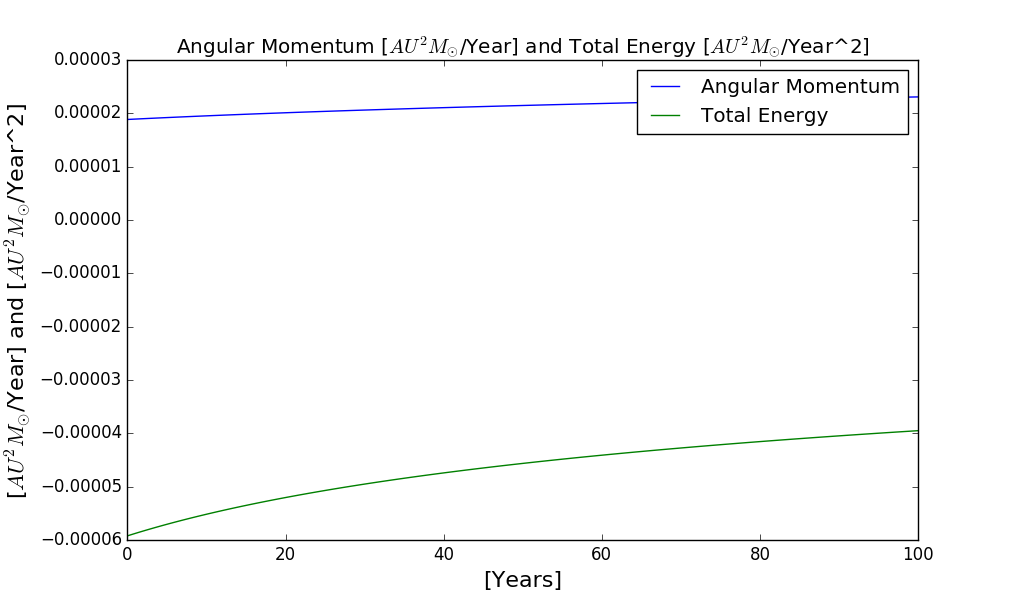
\includegraphics[width=1.1\linewidth]{conserved_euler_J.png}
  \caption{Euler metoden gir ikke bevaring.}
  \label{ang1}
\end{subfigure}%
\begin{subfigure}{.55\textwidth}
  \centering
  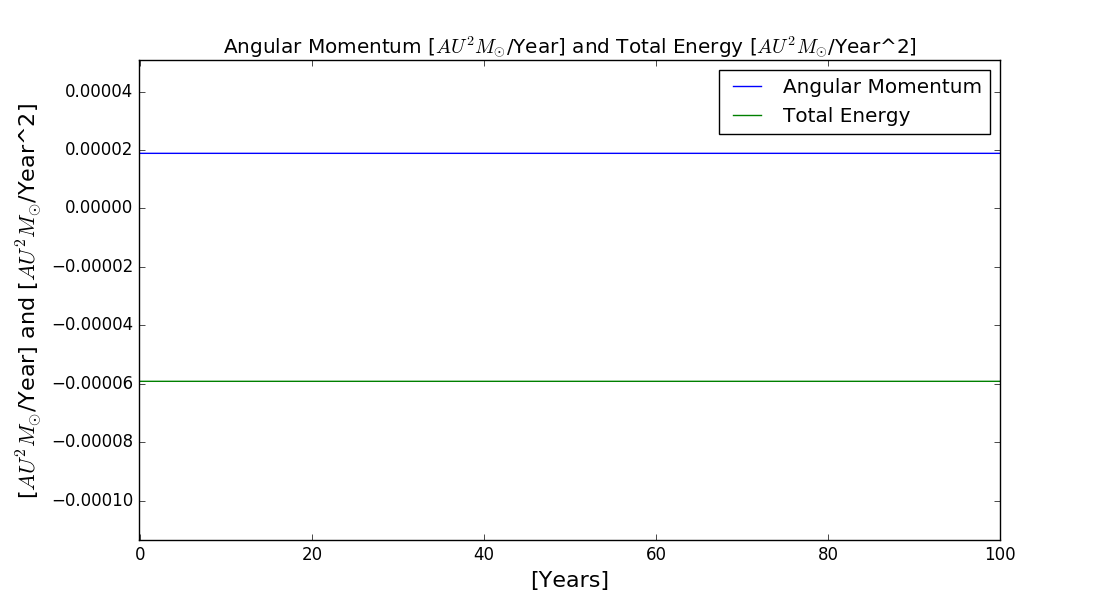
\includegraphics[width=1.1\linewidth]{conserved.png}
  \caption{Velocity Verlet metoden gir god bevaring. }
  \label{ang2}
\end{subfigure}
\caption{Plottet viser Jordas angulærmoment og total mekanisk energi over et århundre. Det er lett å se at både angulærmoment og energi er bevart i velocity Verlet metoden. I Eulers metode er disse verdiende økende.}
\label{fig:duhhhhhh}
\end{figure}
\FloatBarrier
Etterhvert som man zoomer inn på grafene vil man observere oscilleringer av energien og angulærmomentet. I trelegemeproblemet dukker disse opp, selv i VV algoritmen.
Se figur \ref{ang3}. Her ser du hvordan Jupiter tukler med VV's evne til å bevare energi. Dette er sikkert grunnet avrundingsfeil og gjennomsnittet synes å være konstant og ikke-økende.\\

\FloatBarrier
\begin{figure}[!ht]
 \centering
 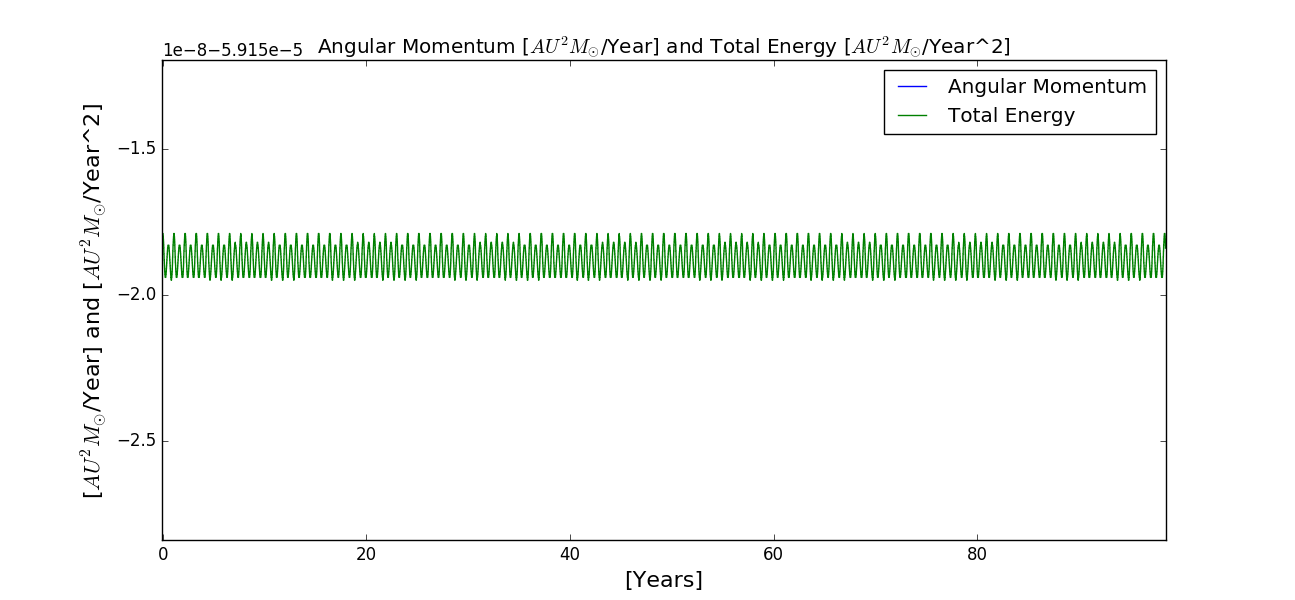
\includegraphics[scale=0.4]{wat.png}
 \caption{Jordas energi i 3-legeme problemet. Datamaskinen klarer ikke fremstille energien og angulærmomentet som perfekt konstant. Spesiellt ikke når flere enn 2 legemer er involvert.}
 \label{ang3}
 \end{figure}
 \FloatBarrier
 
Hvis ikke angulærmomentet og energien er konservert så vil legemene i solsystemet vår bremse/aksellerere uten at vi ønsker det. Euler egner seg derfor ekstremt dårlig til dette prosjektet, mens Velocity Verlet er ideelt.

\subsection{CPU-tid og FLOPS}
Ved å telle antall FLOPS i koden vi har brukt, fant vi ut at antall FLOPS gikk som $N\cdot 29$ i Eulers metode, og $N\cdot 58$  
i velocity Verlet metoden (Akkurat dobbelt så mange). Vi har her funnet CPU-tiden for $dt$=0.001 for ulike antall tidssteg (\texttt{numTimesteps} i koden). Figur \ref{CPU} viser resultatene. Siden CPU-tiden vil forandre seg litt for hver gang vi måler, har vi målt ti ganger for hver \texttt{numTimesteps} og funnet gjennomsnittet av disse verdiene. 

\FloatBarrier
\begin{figure}[!ht]
 \centering
 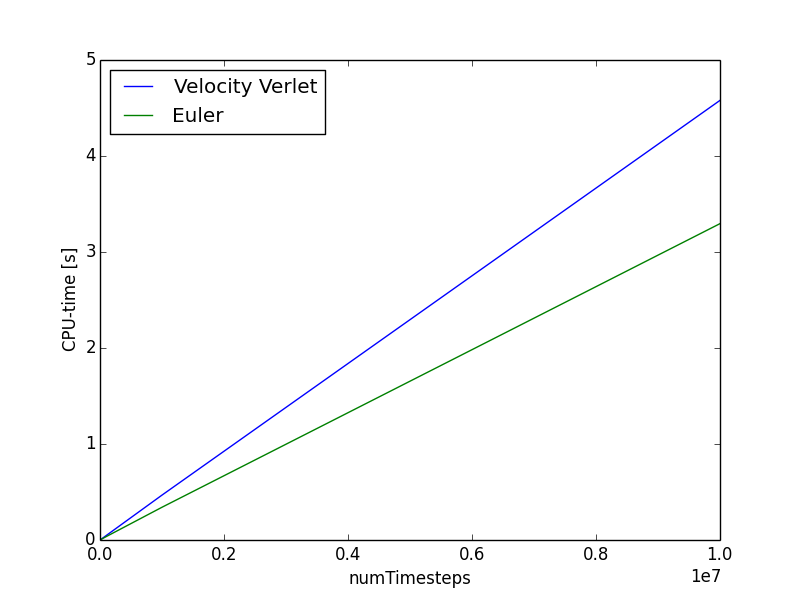
\includegraphics[scale=0.5]{CPU.png}
 \caption{CPU-tiden for de to ulike metodene når dt=0.001. Det er lett å se at velocity Verlet er mer tidkrevende enn Eulers metode, noe som stemmer godt overens med antall FLOPS denne metoden krever i forhold til Eulers metode.}
 \label{CPU}
 \end{figure}
 \FloatBarrier


\subsection{Feil}
Feilen i jordens bane er som den skal være mtp. metodenes skarphet.
Feil måler vi som en funksjon av integrasjonstidssteget sin størrelse (dt $=$ h $= 0.1, \ 0.01, ...$).
Som tidligere gjennomgått har Euler en lokal feil $O(h^{2})$ og en global feil på $O(h^{1})$.
Velocity Verlet har derimot en global feil på $O(h^{2})$. Ved å plotte hver metodes akkumulerte feil forventer vi da en lineær og en andregrads vekst fra hver av dem.
I figur \ref{feil_euler} og \ref{feil_verlet} er de globale feilene i jordas bane plottet for diverse tidssteg mellom $h=10^{-1}$ til $h=10^{-4}$ over ett jordår.\\

\FloatBarrier
\begin{figure}[!ht]
\centering
\begin{subfigure}{.5\textwidth}
  \centering
  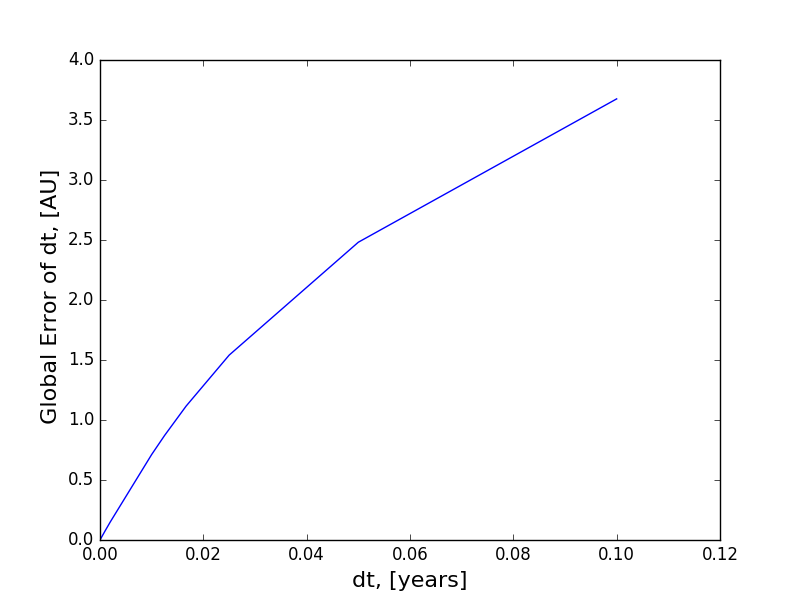
\includegraphics[width=1.1\linewidth]{Euler_Global.png}
  \caption{Euler metoden gir en slik global feil.}
  \label{feil_euler}
\end{subfigure}%
\begin{subfigure}{.5\textwidth}
  \centering
  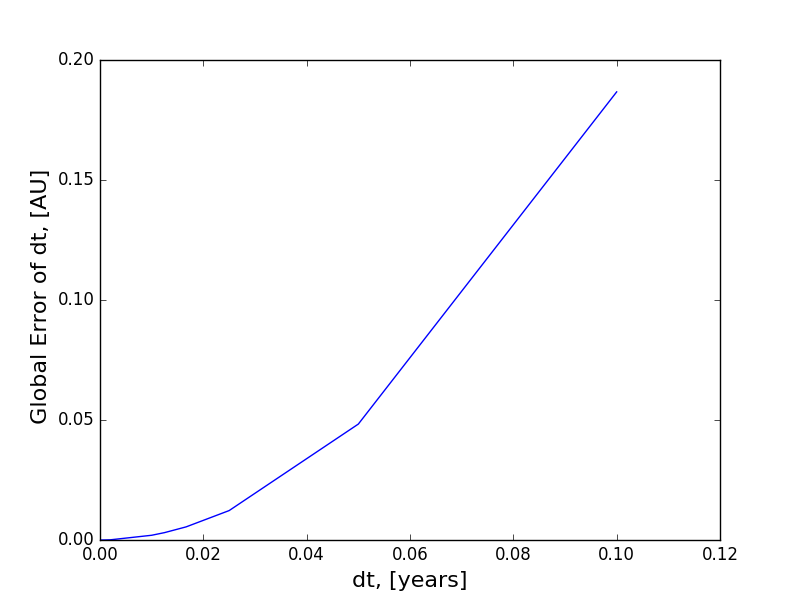
\includegraphics[width=1.1\linewidth]{Verlet_Global.png}
  \caption{Velocity Verlet metoden. }
  \label{feil_verlet}
\end{subfigure}
\caption{Plottet her er den akkumulerte/globale feilen til hver metode når vi måler jordas bane rundt solen, en gang.}
\label{fig:duh}
\end{figure}
\FloatBarrier
Siden feilfunksjonene, $O(h^{p})$, er proporsjonale med $h^p$ kan vi anta at feilfunksjonene er tilnærmet lik $O(h^{p}) \approx \alpha h^p$, der $\alpha$ er en konstant. 
Videre kan vi anta at $\alpha \approx 1$. Nå kan vi si at logaritmen til feilfunksjonene er $\log{\alpha h^p} =p\cdot h$.
 
Dette betyr at stigningtallet til $\log{O(h^{p})}$ er 
$$\frac{d \ \log{O(h^{p})}}{dh} =  p $$ 
Hvis våre metoder stemmer, må altså dette stemme. Logaritmen til feilfunksjonene i \ref{feil_euler} og \ref{feil_verlet} er plottet i 
figur \ref{1swag} og \ref{2swag}.\\

\FloatBarrier
\begin{figure}[!ht]
\centering
\begin{subfigure}{.5\textwidth}
  \centering1
  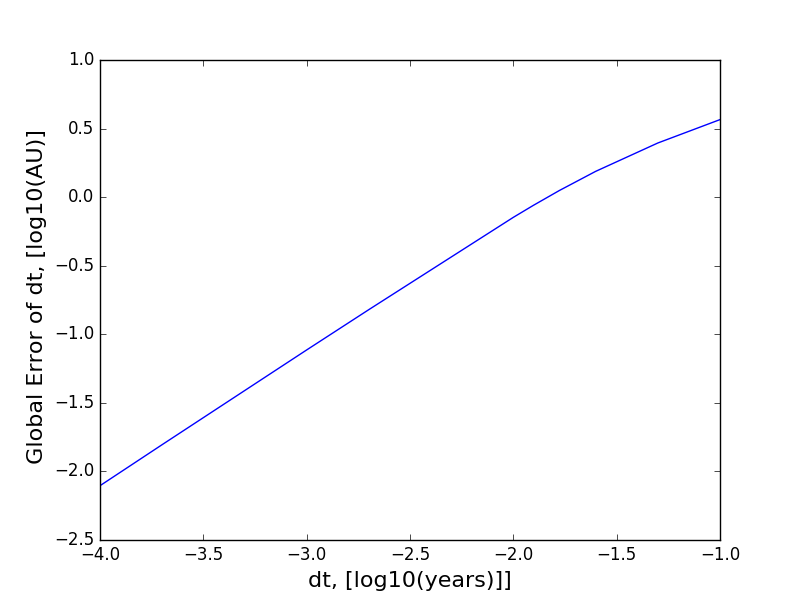
\includegraphics[width=1.1\linewidth]{Euler_Global2.png}
  \caption{Euler metoden, logaritmen av den globale feil.}
  \label{1swag}
\end{subfigure}%
\begin{subfigure}{.5\textwidth}
  \centering
  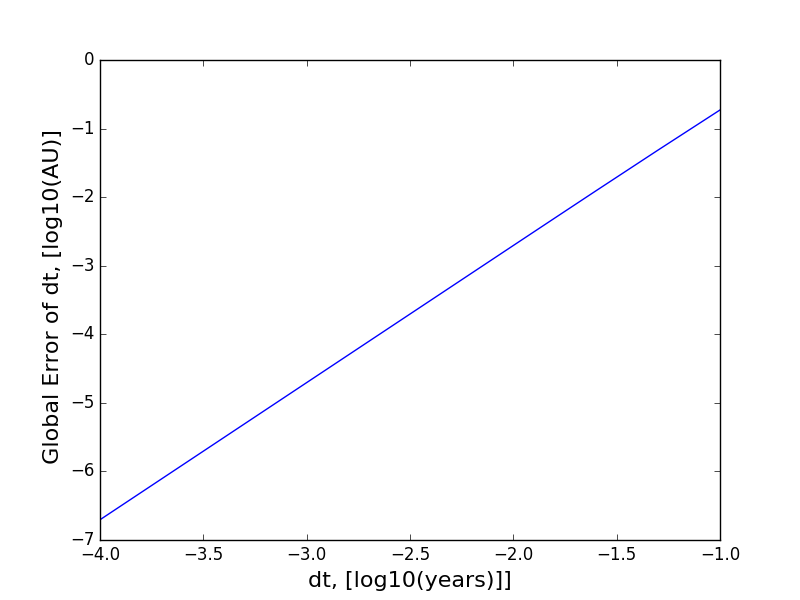
\includegraphics[width=1.1\linewidth]{Verlet_Global2.png}
  \caption{Velocity Verlet metoden. }
  \label{2swag}
\end{subfigure}
\caption{Her ser du tierlogaritmen til de globale feilene. Deres stigning skal være 1 og 2 hver for seg.}
\label{fig:duhh}
\end{figure}
\FloatBarrier
Vi ser her at stigningstallet til Euler metoden er tilnærmet lik 1 (0.89), akkurat som feilgraden ($O(h^{1})$). Logaritmen av VV-metoden, med en feilgrad på 2, har her stigningstall 2 (1.99)! Altså er feilen som den skal være  ($O(h^{2})$).

\subsection{Unnslipningshastighet}
Ved hjelp av prøving og feiling, fant vi unnslipningshastigheten til jorden i en avstand 1 AU fra solen. Dette ble gjort ved å sette jordens posisjon lik $(1,0,0)$ og hastighet $(0,v_y,0)$. Ved å variere verdien til $v_y$ fant vi at unnslipningshastigheten må ligge et sted mellom $v_y$ = 8.75 AU/yr og $v_y$ = 8.90 AU/yr, se figur \ref{fig:uh}. 

\FloatBarrier
\begin{figure}[!ht]
\centering
\begin{subfigure}{.5\textwidth}
  \centering
  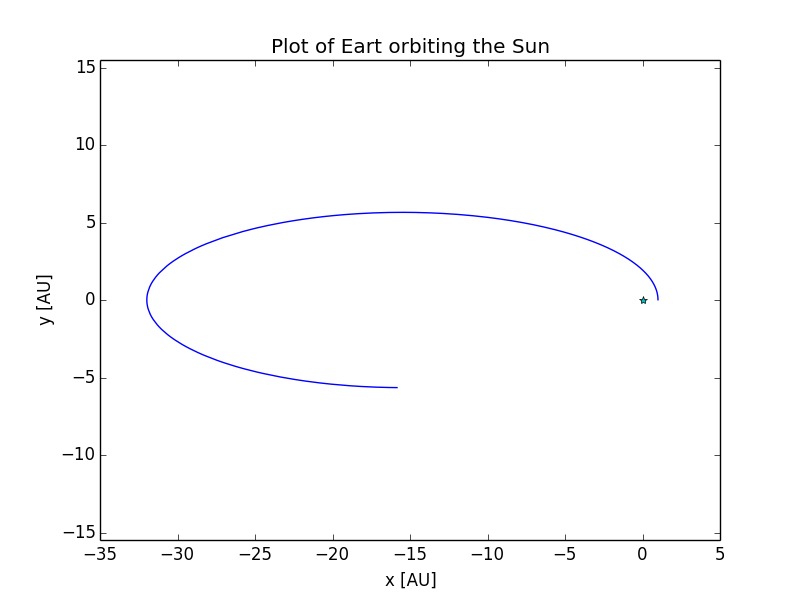
\includegraphics[width=1.1\linewidth]{3d_escape_v_8_75.png}
  \caption{$v_y$ = 8.75 AU/yr}
  \label{fig:sub1}
\end{subfigure}%
\begin{subfigure}{.5\textwidth}
  \centering
  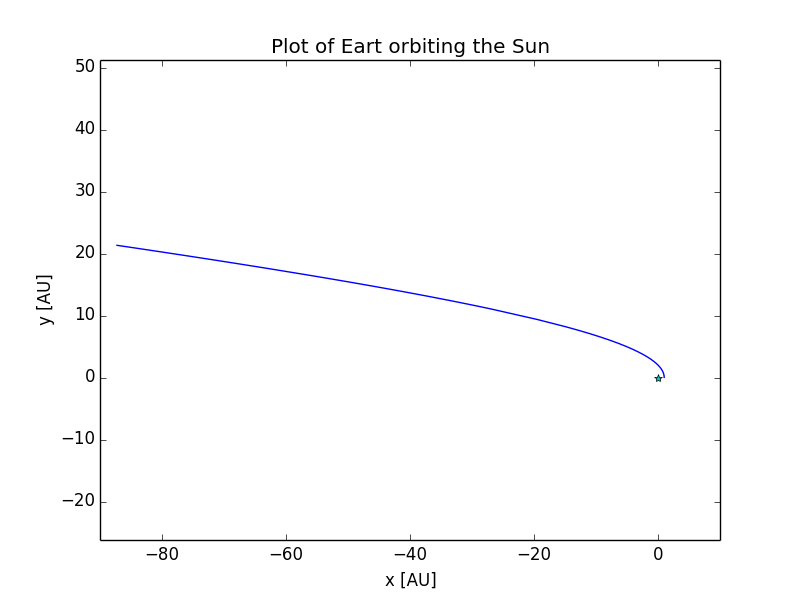
\includegraphics[width=1.1\linewidth]{3d_escape_v_8_9.png}
  \caption{$v_y$ = 8.90 AU/yr}
  \label{fig:sub2}
\end{subfigure}
\caption{Figurene viser jordens bane for ulike unnslipningshastigheter. Vi ser at denne hastigheten må ligge et sted mellom 8.75 og 8.90 AU/yr. I dette tilfellet er det ingen krefter som virker på solen, og den er markert med en stjerne i origo.}
\label{fig:uh}
\end{figure}
\FloatBarrier

Vi kan finne et eksakt svar ved å bruke formelen for unnslipningshastigheten:
\[v_e = \sqrt{\frac{2GM}{r}} \]
Her er $G$ tyngdeakselerasjonen, $M$ solens masse og $r$ avstanden mellom solen og jorden, som i dette tilfellet er 1 AU. Massen til solen er $M_{\odot}$ = 1, og vi ender opp med
\[\sqrt{ \frac{2 \cdot 4\pi^2 \cdot 1 }{1}  } \approx 8.89 \quad AU/yr \]

\subsection{Trelegemeproblemet}
Vi skal nå se på et trelegemesystem bestående av jorden, solen og Jupiter. Solen er fortsatt systemets massesenter slik at den står stille i vår modell. Jupiter er den mest massive av alle planetene i solsystemet, og vil påvirke jordens bane rundt solen med sin tyngdekraft:
\[F_{Earth-Jupiter} = \frac{GM_{Jupiter}M_{Earth}}{r^2_{Earth-Jupiter}} \]

Ved å legge til planeten Jupiter i programmet vårt, kan vi enkelt se hvordan  tyngdekraften som virker mellom jorden og Jupiter påvirker jordas bane. Figur \ref{jupiterx1} viser posisjonen til jorden og Jupiter.

\FloatBarrier
\begin{figure}[!ht]
\begin{center}
  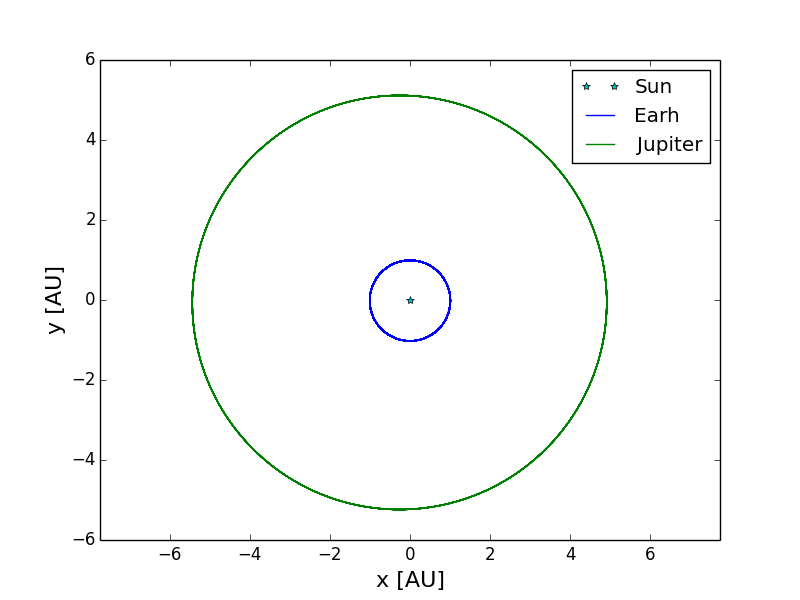
\includegraphics[width = 100mm]{jupiterx1.png}\\
  \caption{Plot av jordens og Jupiters bane rundt solen. Her er Jupiters masse omtrent en tusendedel av solens masse, og vi ser at jordens bane ikke påvirkes nevneverdig.}   \label{jupiterx1}
  \end{center}
  \end{figure}
\FloatBarrier

Vi brukte velocity Verlet metoden for å plotte banen til jorden og Jupiter. Figur \ref{stabilitetJ1} viser stabiliteten til løsningen vi fikk ved å bruke velocity Verlet metoden. Vi har her sammenlignet jordens bane under påvirkning fra Jupiters masse med hvordan jorden ville ha beveget seg uten Jupiter (en perfekt sirkel). \\

\FloatBarrier
\begin{figure}[!ht]
\begin{center}
  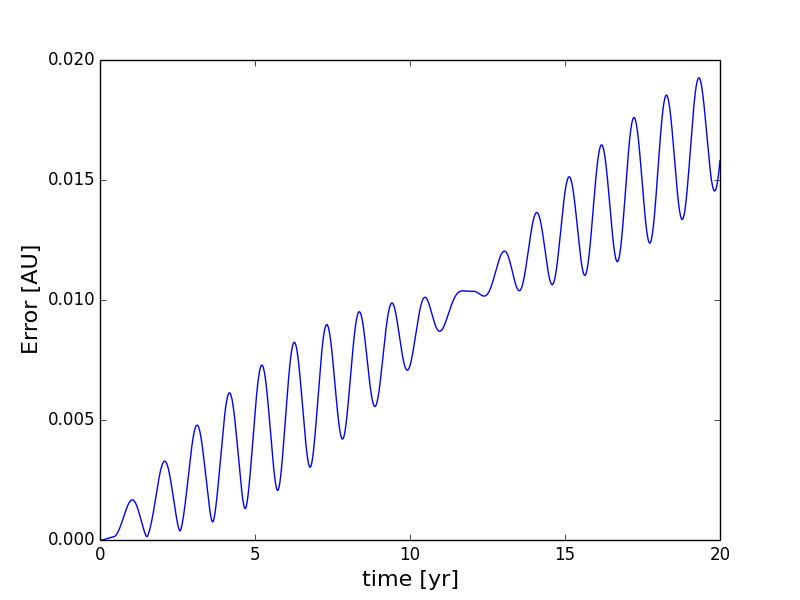
\includegraphics[width = 100mm]{3e_error_dt_e-3.png}\\
  \caption{Vår simulerte jordbanes avstand fra en perfekt sirkelbane under påvirkning av Jupiter.}   \label{stabilitetJ1}
  \end{center}
  \end{figure}
\FloatBarrier
Som du ser gir velocity verlet en løsning som aldri viker lenger enn en gitt avstand. Dette gjør den overlegen og setter Euler i skyggen, som har en løsning som viker mer og mer fra den ideelle sirkelbane.

Dersom vi øker massen til Jupiter med en faktor 1000,  \ref{jupiterx1000}

\FloatBarrier
\begin{figure}[!ht]
\begin{center}
  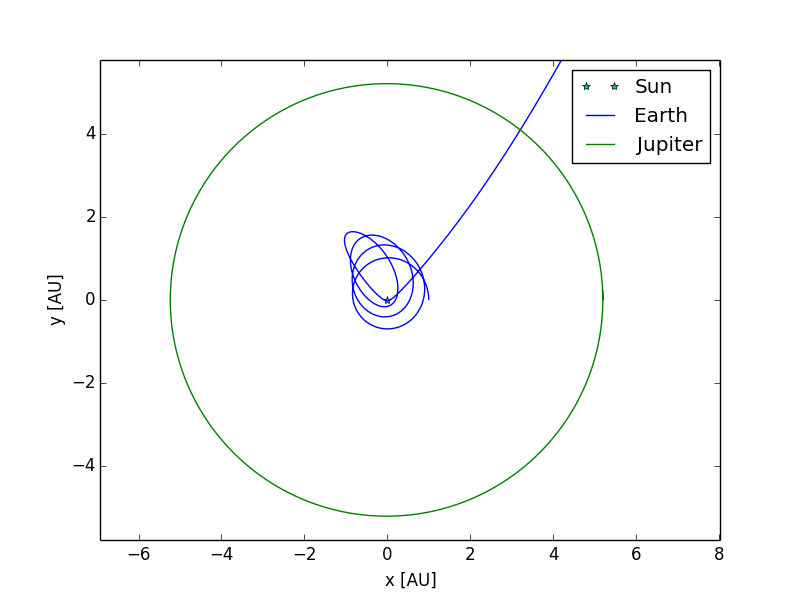
\includegraphics[width = 100mm]{jupiterx1000.png}\\
  \caption{Plot av jordens og Jupiters bane rundt solen. Her er Jupiters masse økt med en faktor 1000, slik at den nesten har samme masse som solen. Tyngdekraften som virker mellom jorden og Jupiter vil derfor være mye større, og jordens bane vil påvirkes av dette. Den går noen ustabilde runder rundt solen før den slynges ut i verdensrommet. }   \label{jupiterx1000}
  \end{center}
  \end{figure}
\FloatBarrier

Når vi utvider fra Sol-Jord systemet til hele solsystemet vil vi ikke lenger holde solen fikset i origo. Vi beregner istedet posisjonen til massesenteret. Deretter defineres systemets origo her. Vi gir så solen en initial hastighet i bane rundt massesenteret 
mtp. at systemets nettomoment ikke skal overstige null.	\\

Posisjonen til massesenteret er summen av legemenes posisjonen vektet med hvert av legemes masse, delt på totalmassen til solsystemet. Vi inkluderer solen, solen er ikke lenger origo.
\begin{equation}
 \vec{R}_{cm} = \sum_i \frac{\vec{r_i}m_i}{M_{tot}}
\end{equation}
De nye startposisjonene til legemene blir da $$\vec{r}_{new} = \vec{r}_{before} - \vec{R}_{cm}$$
For at systemet vårt ikke skal vandre vekk må massesenteret være stillestående, noe som betyr at bevegelsesmengden til massesenteret $\vec{P}_{cm} = 0$.
Dette kan raskt implementeres ved å beregne alle legemenes bevegelsesmengde og gi sola denne bevegelsesmengden i motsatt retning. Eller med andre ord, gi sola en fart i motsatt retning.
\begin{equation}
 \vec{v}_{\odot} = -\sum_i \frac{m_i\vec{p}_{i}}{M_{\odot}}
\end{equation}



\subsection{Endelig modell med alle planeter i solsystemet}
I figur \ref{all} viser et plot av hvordan systemet utvikler seg som funksjon av tid når vi har med alle planetene i solsystemet. Avviket i jordens bane rundt solen vises i figur \ref{all_error}. 

\FloatBarrier
\begin{figure}[!ht]
\begin{center}
  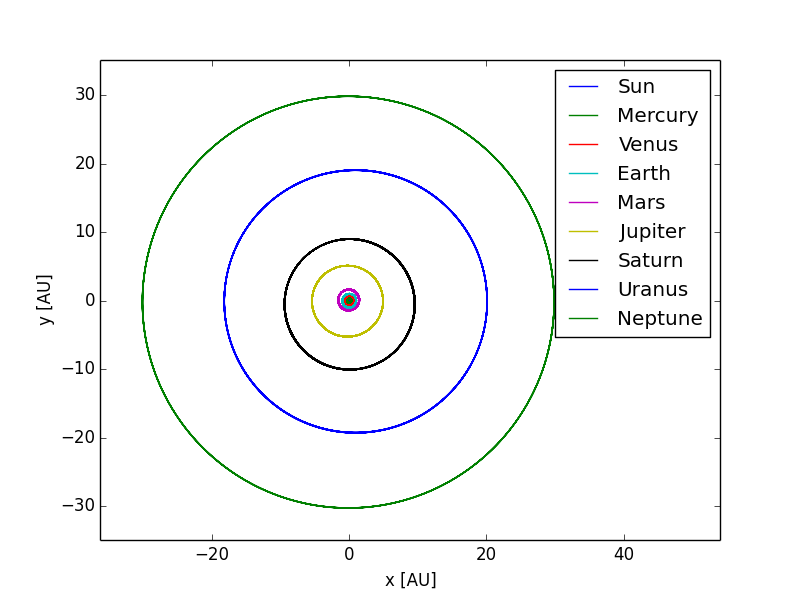
\includegraphics[width = 120mm]{3f_all.png}\\
  \caption{Vårt fullstendige solsystem med alle planeter inkludert.}   \label{all}
  \end{center}
  \end{figure}
\FloatBarrier

\FloatBarrier
\begin{figure}[!ht]
\begin{center}
  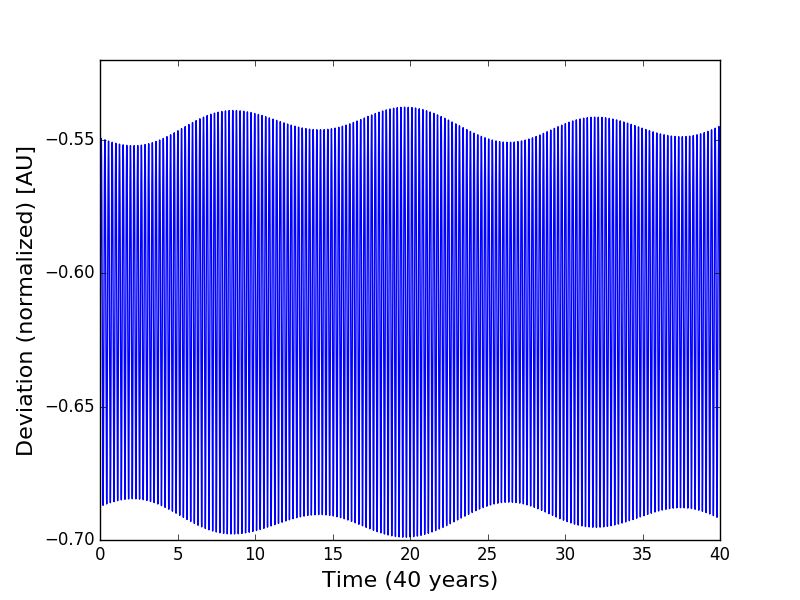
\includegraphics[width = 100mm]{solar.png}\\
  \caption{Vår simulerte jordbanes avstand fra en perfekt sirkelbane under påvirkning av alle planetene i solsystemet.}   \label{all_error}
  \end{center}
  \end{figure}
\FloatBarrier
Selv når hele solsystemet drar på jorda klarer velocity Verlet å holde jorda innenfor en konstant rekkevidde langs den idelle banen, uansett hvor lang tid som går forbi (figur \ref{all_error}).

\subsection{Merkurs perihelpresesjon}
Presesjon er et fysisk fenomen som vil vise seg når aksen til et roterende objekt "slingrer" mens det utsettes for en ytre kraft. Dette viser seg å gjelde for planetene i solsystemet vårt også. Vi kan se på presesjonen som en langsom endring i rotasjonsaksens retning for et legeme som roterer og samtidig påvirkes av en ytre kraft, i vårt tilfelle tyngdekraften. I virkeligheten er ikke en planets bane rundt solen ellipseformet. Dersom vi lar planeten gå mange nok runder rundt sola, vil vi kunne se at banen heller er kronblad-formet. Dette kommer av at aksen til planetens elliptiske bane preseserer, slik at vi får en langsom endring i rotasjonsaksen. Det er mulig å observere størrelsen på Merkurs perihelpresesjon. Sammenligner vi disse observasjonene med perihelpresesjonen beregnet ved klassisk mekanikk, finner vi et avvik. Dette avviket ble spådd av Einsteins relativitetsteori, og er et viktig eksperimentellt resultat som førte til at den generelle relativitetsteorien ble allment akseptert [8]. Gjennom den generelle relativitetsteorien får vi altså et nytt ledd i Newtons tyngdelov: 

\begin{equation}
F_G = \frac{GM_{\odot}M_{Mercury}}{r^2}\left[1 + \frac{3l^2}{r^2c^2} \right]
\end{equation}

hvor $r$ er avstanden mellom Merkur og solen, $c$ er lysets hastighet og $l = |\vec{r}x\vec{v}|$ er størrelsen på Merkurs angulærmoment per masse. Vi kan finne vinkelen på Merkurs perihel ved 
\[tan \theta_p = \frac{y_p}{x_p} \]
hvor $x_p$ og $y_p$ er forholdsvis $x$ og $y$ koordinaten til Merkurs posisjon ved perihelion, som er punktet der Merkur er nærmest solen.

Presesjonen vi observerer over 100 jordår hos Merkurs perihelion, gitt at bare sola og Merkur vekselvirker kraftmessig, er på 43 buesekunder ($43/3600$ grader $= 43''$).
For å simulere dette riktig trengte vi tidssteg på ca. $10^{-8}$år. Da fikk vi en veldig god tilnærming på $42.93''$! Se figur \ref{arc1}. Når vi fjerner GR korreksjonen vil perihelion oscillere, se figur \ref{arc2}.\\

\FloatBarrier
\begin{figure}[!ht]
\centering
\begin{subfigure}{.5\textwidth}
  \centering
  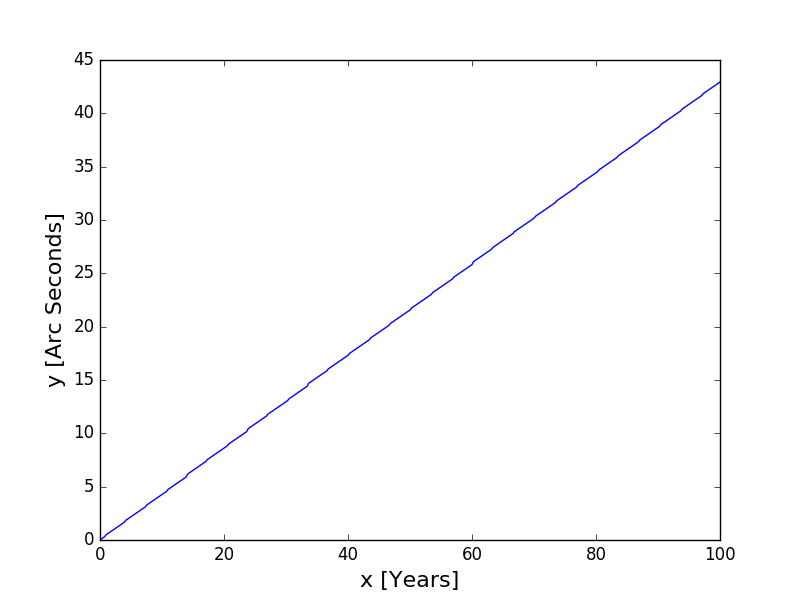
\includegraphics[width=1.1\linewidth]{arcs1.png}
  \caption{Med GR korreksjon, 100 år, h$ = 10^{-8}$år}
  \label{arc1}
\end{subfigure}%
\begin{subfigure}{.5\textwidth}
  \centering
  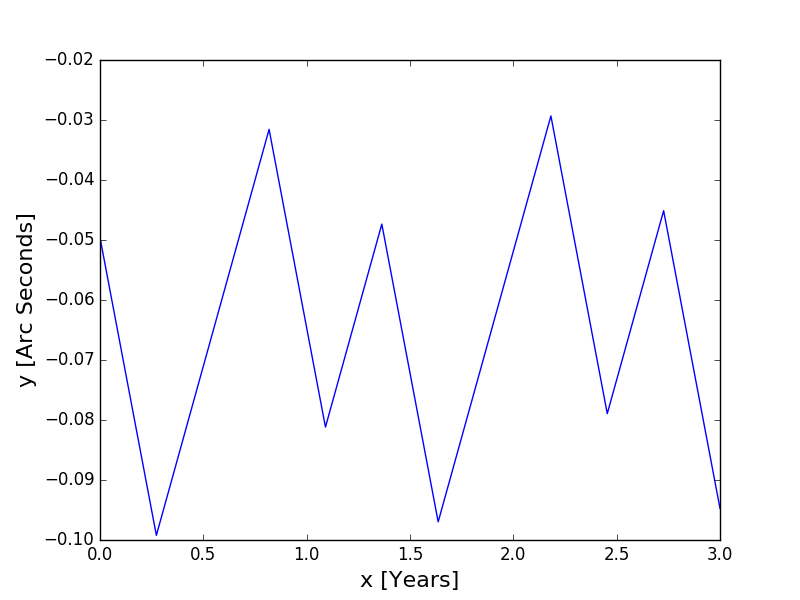
\includegraphics[width=1.1\linewidth]{arcs2.png}
  \caption{Uten GR korreksjon, 3 år, h$ = 10^{-8}$år}
  \label{arc2}
\end{subfigure}
\caption{Figurene viser Merkurs perihelionspresesjon i buesekunder. Uten korreksjonsleddet fra GR har vi ingen merkbarlig presesjon.}
\label{fig:uh}
\end{figure}
\FloatBarrier

Perihelionspresesjonen uten GR er uordnet. Det er nok ikke så kaotiskt i virkeligheten, men siden feil bygges opp, selv i velocity Verlet, vil ikke presisjonen være perfekt. Ser vi på middelverdien av kaoset i figur \ref{arc2} kan vi anta at
perihelion ikke endrer seg sedvanlig. 

\section{Diskusjon og konklusjon}
Dersom vi ser konserveringen av jordas angulærmoment, som vises i figur \ref{ang1} og \ref{ang2}, er det lett å se at velocity Verlet metoden er å foretrekke. Både totalenergien og angulærmomentet holder seg konstant, noe som betyr at disse størrelsene er bevart som funksjon av tid. Som tidligere nevnt er ikke Euler den mest nøyaktige løsningsmetoden vi har, og figur \ref{ang1} bekrefter dette. I figur \ref{ang3} ser vi et lite utsnitt av grafen til energien i velocity Verlet løsningen. Her kunne vi se at energien oscillerte, og det samme gjaldt også for angulærmomentet. Dette kan komme av at Jupiter påvirker metodens evne til å bevare energi og angulærmoment, som kan lede til avrundingsfeil. Likevel er gjennomsnittet av de oscillerende grafene konstant og vi har bevaring av energi og angulærmoment i velocity Verlet metoden. Vi hadde derfor god grunn til å fortsette bruken av denne metoden i resten av prosjektet. \\

Som sagt har Eulers metode en global feil på $O(h)$, mens velocity Verlet metoden har en global feil på $O(h^2)$. I plottene \ref{feil_euler} og \ref{feil_verlet} ser vi hvordan feilen i de to metodene går som funksjon av tidssteget $dt$. Vi ser at plottene svarer til det vi kan forvente; feilen i Eulers metode går som en lineær funksjon, mens feilen i velocity Verlet metoden går som en andregradsfunksjon. 

Vi har sett at velocity Verlet metoden hadde dobbelt så mange FLOPS som Eulers metode, og dette kom til syne når vi målte CPU-tiden til de to metodene. Her var det tydelig at velocity Verlet metoden krevde mer CPU-tid enn Eulers metode. Likevel vil velocity Verlet metoden være å foretrekke, da denne er mye mer stabil på lang sikt. Hvis man antar at hver FLOP bruker like lang tid, skulle en tro at velocity Verlet metoden ville bruke dobbelt så lang tid som Euler. I følge plottet i figur \ref{CPU} er ikke verden like svart og hvit. Grunner til dette er at hver FLOP faktisk ikke bruker like lang tid på å utføres. I tillegg er det mulig vår kompilator er smartere enn vi tror, selv om vi ikke har tatt i bruke såkalte "flags" for å gjøre prosessen raskere.\\

Den eksperimentelt funnede unnslipningshastigheten stemmer godt overens med den eksakte løsningen. Da vi anslo at $v_e$ måtte ligge i intervallet $<$8.75, 8.90$>$, fikk vi en eksakt løsning på $8.89$ AU/yr. Dette viser at koden vår ser ut til å fungere i henhold til de fysiske lovene.\\

Da vi innføre Jupiter fikk vi se hvordan dens masse kom til å påvirke jordens bane med sin tyngdekraft. Vi ser i figur \ref{jupiterx1} at jorden fortsetter å gå i bane rundt solen, som forventet. Dersom vi ser nærmere på avviket i banen fra en perfekt sirkel, som vist i figur \ref{stabilitetJ1}, vil vi se at avviket ikke øker som funksjon av tid, men alternerer heller mellom omtrent -0.010 AU og 0.025 AU. Hver periode tilsvarer ett jordår, mens perioden til \textit{omhyllingskurven} tilsvarer ett jupiterår. Dette viser igjen stabiliteten i velocity Verlet metoden vi bruker. I figur \ref{jupiterx1000} ser vi hva som ville skjedd dersom Jupiters masse var like stor som solmassen. Da ville jorden blitt påvirket sterkt av jupiters tyngdekraft, noe som resulterer i at jorden slynges ut i det store intet. \\

Når vi har et fullt solsystem med alle planeter til stede, får vi en litt annen kurve for jordbanens avvik fra en sirkel. Denne gangen er det ikke bare Jupiter som drar i jorden med sin tyngdekraft, og vi ser at spennet her er mye større. Alterneringene skjer mellom -0.70 AU og -0.55 AU. Dette gir mening, da det er mange flere planeter som påvirker jorden.\\

Etter at vi innførte et korreksjonsledd som konsekvens av generell relativitet til Merkurs vekselvirkning med sola, dukket perihelionpresesjon opp. Uten korreksjonsleddet var denne presesjonen for liten til å måles over bare 3 år. Konsekvensene av GR som vi er kjent med er bremsing av tid ved tyngdefelt, relativt til der det ikke er tyngdefelt. Dette forteller oss at det kanskje oppstår en forlengelse av tid i nærheten av sola, relativt til lenger vekke fra sola. Derfor observerer vi det som om Merkur beveger seg litt mer enn den egentlig burde få lov til og som konsekvens får den en presesjon i både perihelion og aphelion.


\section{Vedlegg}
Alle koder og resultater som er brukt i rapporten finnes på Github-adressen: \\
https://github.com/livewj/PROJ3


\bibliography{Referanser}
\begin{thebibliography}{9}  

\bibitem{}
  Kursets offisielle Github-side $\textit{FYS3150 - Computational Physics}$
  https://github.com/CompPhysics/ComputationalPhysics,
  19.10.2016  
    
\bibitem{}
   M. Hjort-Jensen: Computational physics, lecture notes 2015. Fysisk institutt, UiO, 2016.

\bibitem{}
   Oppgavetekst: Project 3, Fysisk institutt, UiO, 19.10.16
   
\bibitem{}
    "solar-system-fys3150"
    https://github.com/mortele/solar-system-fys3150
    19.10.2016
    
\bibitem{}
    Tyngdekraft
    https://no.wikipedia.org/wiki/Tyngdekraft
    19.10.2016
\bibitem{}
    HORIZONS Web-Interface: http://ssd.jpl.nasa.gov/horizons.cgi$\#$top
    13.10.2016
    
\bibitem{}
  Slides fra kursets offisielle nettside
  "Ordinary differential equations":
  http://compphysics.github.io/ComputationalPhysics/doc/pub/ode/pdf/ode-beamer.pdf, 21.10.16
  
  \bibitem{}
  "Presesjon"
  https://no.wikipedia.org/wiki/Presesjon, 21.10.16
   
\end{thebibliography}
\end{document}


